\section{Experimental Results}
\label{sec:lab}

We were able to build the circuit presentially utilizing a breadboard and the various components.

Then, the frequency of the input voltage source was ajusted, from $50 Hz$ to $50 kHz$, at various increments and, for each value, the value of the output voltage was measured.
The results are in the following table:

\begin{table}
    \caption{Gain as a function of frequency}
    \vspace{-3mm}
    \begin{tabular}{|c|c|}
    \hline
    f(Hz) &  V_L(mV)\
    $50.0$  &   $98$\
    $75.0$  &   $133$\
    $100.0$ &  $173$\ 
    $125.0$ &  $209$\
    $150.0$ &  $249$\
    $200.0$ &  $318$\ 
    $225.0$ &  $346$\
    $250.0$ &  $378$\ 
    $275.0$ &  $406$\
    $300.0$ &  $440$\
    $325.0$ &  $462$\
    $350.0$ &  $500$\
    $375.0$ &  $520$\
    $400.0$ &  $540$\
    $450.0$ &  $580$\
    $500.0$ &  $610$\
    $550.0$ &  $640$\ 
    $600.0$ &  $670$\ 
    $700.0$ &  $710$\
    $800.0$ &  $720$\
    $900.0$ &  $730$\
    $1000.0$ &  $740$\
    $1100.0$ &  $720$\
    $1200.0$ &  $720$\ 
    $1300.0$ &  $710$\ 
    $1400.0$ &  $690$\
    $1500.0$ &  $680$\
    $1600.0$ &  $660$\
    $1700.0$ &  $640$\
    $1800.0$ &  $630$\
    $1900.0$ &  $610$\ 
    $2000.0$ &  $590$\ 
    $2200.0$ &  $540$\
    $2600.0$ &  $510$\
    $3000.0$ &  $470$\
    $3300.0$ &  $430$\
    $3600.0$ &  $400$\
    $3900.0$ &  $380$\ 
    $4200.0$ &  $350$\ 
    $4500.0$ &  $330$\
    $5000.0$ &  $300$\
    $5500.0$ &  $277$\
    $6000.0$ &  $257$\
    $6500.0$ &  $241$\
    $7000.0$ &  $225$\ 
    $7500.0$ &  $213$\ 
    $8000.0$ &  $197$\
    $9000.0$ &  $181$\
    $10000.0$&  $165$\
    $12000.0$ &  $141$\
    $15000.0$ &  $117$\
    $20000.0$ &  $88$\ 
    $50000.0$ &  $38$\ 

    \hline
    \end{tabular}
    \label{tab:fvl}
\end{table}

    These results were graphed below as to compare them to the theoretical analysis and simulation done above:

    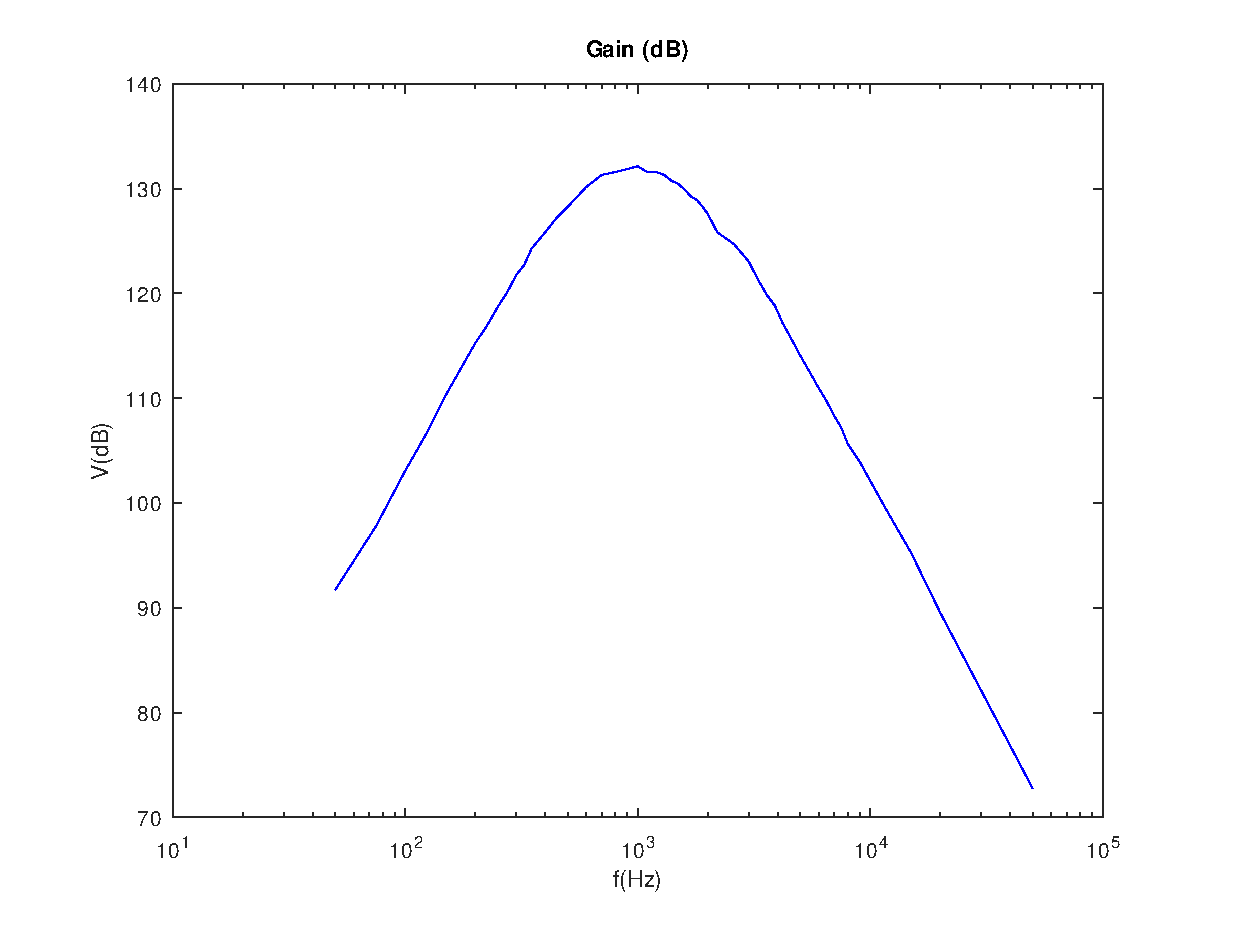
\includegraphics[width=1\linewidth]{lab.eps}